
\section{Software Testing}

	The goal of testing software is to provide information about the quality of the product. 
	It allows developers to know about potential bugs but it also allows the business to appreciate more the product by giving them some 
documents with the applcation's functionalities. \\  

The company has a quite big application and they have some code that they didn't develop. So we had to do a lot of software testing in order to know all
the bugs of the application. 
I wil start to give you an example of test I had to do and an example of bug I found. 
When we used the school bag service and we click on the button new Folder and click on the close button. Then we couldn't
click again on the new Folder button. \\
I also had to test more complicated services such as the coherence between 
teacher, parents and students accounts. For example if a teacher add
an homework for a class, all the sudents should see it as well as their parents. \\

But doing some tests without writing anything about them is not very useful for the future of the company. That's why I test all the services of the application and report about all the functionalities of every services on a 
document test. I learnt how to write lisable tests documents and it is not so obvious.  

	 In this part I will describe my different tasks in software testing. 
	 I separate software testing in two parts that represent my work: Acceptance testing and Resgression testing. So I will first descibe these two kind of testing and explain what I did for the company. 
	 In the last part I will focus on a software that I used a bit for testing : JMeter.  \\

\newpage
\subsection{Acceptance testing}
I named this section Acceptance testing but I will more talk about how to 
write a technical validation report than testing. 

Individual software modules are combined and tested as a group. The purpose
of these tests is to "proove" that the application meets its requirement. So it consists of verifying functional, performance and reliability requirements. 
My task was to test all the functionalities of the application and report them all in a technical validation report. This document is a measuring tool
which will be very useful to do regression tests. 
As the application is suposed to work in all web browser that the customers
would be likely to use, I had to test the functionalities on these web
browsers. I finally did it on three of them : Firefox, Google chrome and
Internet Explore in Window.   
I will give you a detailed example about the wysiwyg editor : \\ 
\begin{itemize}
	\item Access to the service

\begin{tabular}{|m{4cm}|m{3cm}|m{4cm}|m{2.1cm}|}
\hline
\textbf{Name of the stage} & \textbf{Description}
 & \textbf{Expected result} & \textbf{Comments} \\
\hline
Select Schoolbag service then the Create menu -> Document & 
Opening of the editor Wysiwyg & 
\begin{minipage}{0.7\textwidth}
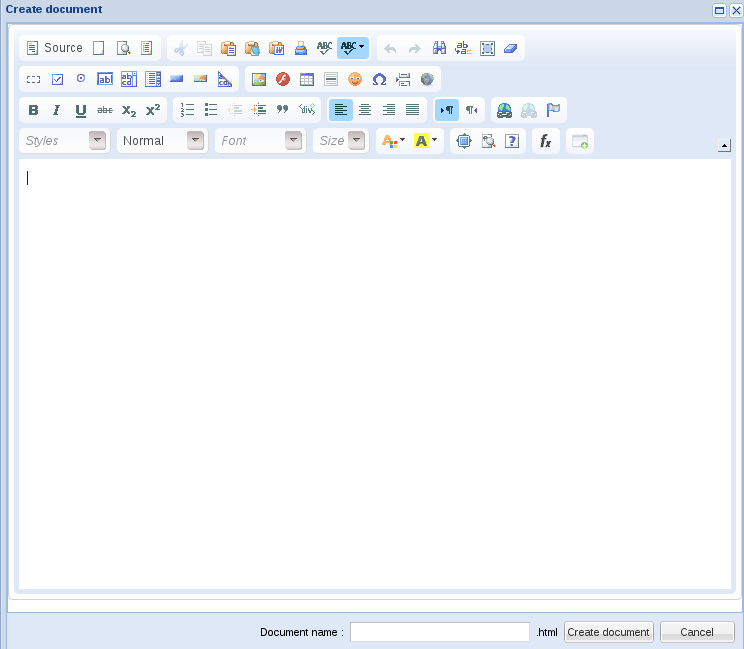
\includegraphics[scale=0.15]{Images/wysi.png} 
\end{minipage}& 
\\
\hline
\end{tabular}
\\
	\item Create a document

\begin{tabular}{|m{4cm}|m{3cm}|m{4cm}|m{2.1cm}|}
\hline
\textbf{Name of the stage} & \textbf{Description}
 & \textbf{Expected result} & \textbf{Comments} \\
\hline
\begin{enumerate}
	\item Fill a description of a document

	\item Choose a name : test

	\item Select create document 
\end{enumerate}&
Display of the new document in the list : test.html & 
\begin{minipage}{0.7\textwidth}
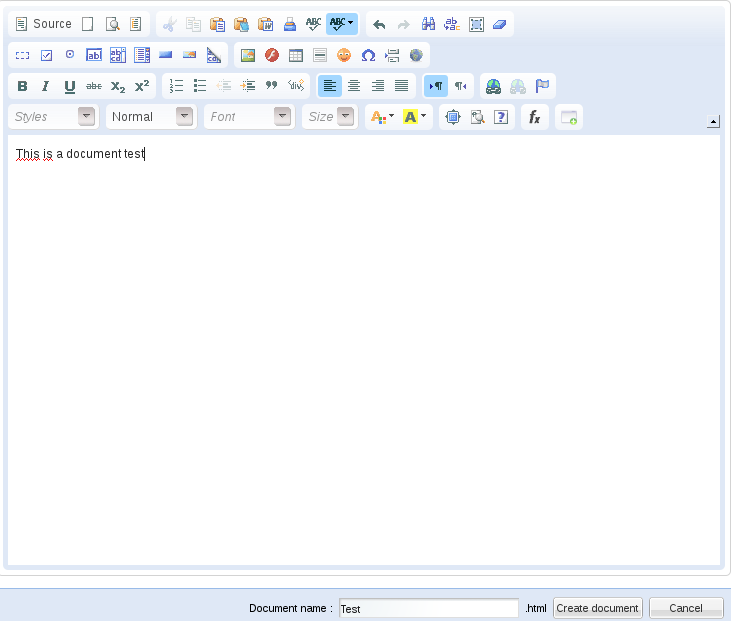
\includegraphics[scale=0.15]{Images/document.png} 
\end{minipage}& 
\\
\hline
\end{tabular}
\\
\end{itemize}

In the document I created one section for each service. Then I accompanied 
each functionalitie with a formal description of the actions to perform, 
the eventual input data and their expected output. 
My descriptions has to be as high level as possible in order to be understanble for the customers. 

\newpage
\subsection{Regression testing}
It is a kind of software testing that consists to uncover new softwares bugs
or regression. These tests are done after some changes such as bugs fixing
or new configurations settings. Indeed, we can manage to fix a bug but 
meanwhile a new bug can appear. So regression testing aim to discover these
kind of new bugs, it helps to determine whether a change in one part of the
 software affects other parts of the software.

Each time the team published changement in the application, I had to do some
regression testing. I run previous set of test-cases by folowing the 
technical validation report. For each test, I compare the results obtained
with the expected results. If there is a correct match for the test,
no new bugs had appeared for this functionalitie. If not, I report the bug in a new Redmine issue.
In these issues I described with precision the bug I detected. It is very 
important to know in which environment the bug had been found such as 
windows or debian, Firefox, Google chrome or Internet Explorer as well as 
all the stages are needed to reproduce the bug.  \\ 

Here is an example of creation of Redmine issue : \\ 

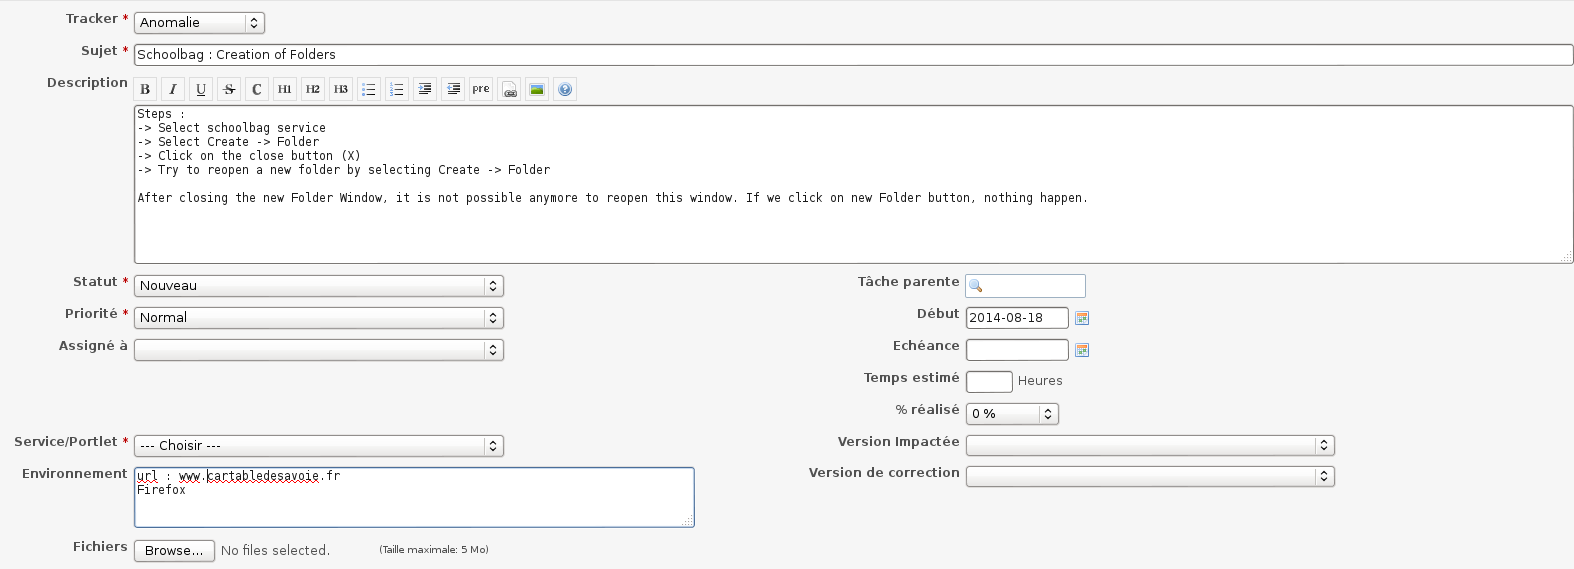
\includegraphics[scale=0.25]{Images/issue.png} 



\newpage
\subsection{JMeter}
\begin{figure}[h]
	
\includegraphics[scale=0.5]{Images/JMeter.jpeg}
	JMeter is a software to test web application.
\end{figure}


